\documentclass[thmsa,11pt,a4paper]{article}

\usepackage{setspace,graphicx,epstopdf,amsmath,amsfonts,amssymb,amsthm}
\usepackage{marginnote,datetime,enumitem,subfigure,rotating,fancyvrb}
\usepackage{hyperref,float}
\usepackage[longnamesfirst]{natbib}
\usepackage{amssymb}
\usepackage{amsmath,amssymb}
\usepackage{titlesec}
\usepackage{mathabx}
\usepackage{pifont}
\usepackage{eurosym}
\usepackage[titletoc,title]{appendix}
\usepackage{tikz}
\usepackage{listings}


\usepackage{booktabs}
\usepackage{hyperref}
\hypersetup{colorlinks,linkcolor={blue},citecolor={blue},urlcolor={blue}}  

\usetikzlibrary{patterns}



\usdate

% These next lines allow including or excluding different versions of text
% using versionPO.sty

%\excludeversion{notes}		% Include notes?
%\includeversion{links}          % Turn hyperlinks on?

% Turn off hyperlinking if links is excluded
%\iflinks{}{\hypersetup{draft=true}}

% Notes options


% Allow todonotes inside footnotes without blowing up LaTeX
% Next command works but now notes can overlap. Instead, we'll define 
% a special footnote note command that performs this redefinition.
%\renewcommand{\marginpar}{\marginnote}%

% Save original definition of \marginpar
\let\oldmarginpar\marginpar

% Workaround for todonotes problem with natbib (To Do list title comes out wrong)
\makeatletter\let\chapter\@undefined\makeatother % Undefine \chapter for todonotes

% Define note commands
\newcommand{\smalltodo}[2][] {\todo[caption={#2}, size=\scriptsize, fancyline, #1] {\begin{spacing}{.5}#2\end{spacing}}}
\newcommand{\rhs}[2][]{\smalltodo[color=green!30,#1]{{\bf RS:} #2}}
\newcommand{\rhsnolist}[2][]{\smalltodo[nolist,color=green!30,#1]{{\bf RS:} #2}}
\newcommand{\rhsfn}[2][]{%  To be used in footnotes (and in floats)
\renewcommand{\marginpar}{\marginnote}%
\smalltodo[color=green!30,#1]{{\bf RS:} #2}%
\renewcommand{\marginpar}{\oldmarginpar}}
%\newcommand{\textnote}[1]{\ifnotes{{\noindent\color{red}#1}}{}}
\newcommand{\textnote}[1]{\ifnotes{{\colorbox{yellow}{{\color{red}#1}}}}{}}

% Command to start a new page, starting on odd-numbered page if twoside option 
% is selected above
\newcommand{\clearRHS}{\clearpage\thispagestyle{empty}\cleardoublepage\thispagestyle{plain}}

% Number paragraphs and subparagraphs and include them in TOC
\setcounter{tocdepth}{2}

% JFE-specific includes:




%\documentclass[thmsa,11pt,a4paper]{article}
%%%%%%%%%%%%%%%%%%%%%%%%%%%%%%%%%%%%%%%%%%%%%%%%%%%%%%%%%%%%%%%%%%%%%%%%%%%%%%%%%%%%%%%%%%%%%%%%%%%%%%%%%%%%%%%%%%%%%%%%%%%%%%%%%%%%%%%%%%%%%%%%%%%%%%%%%%%%%%%%%%%%%%%%%%%%%%%%%%%%%%%%%%%%%%%%%%%%%%%%%%%%%%%%%%%%%%%%%%%%%%%%%%%%%%%%%%%%%%%%%%%%%%%%%%%%
%\DeclareMathOperator{\E}{\mathbb{E}}

\usepackage{amsfonts}
\usepackage{amsmath}
\usepackage{amsthm}
\usepackage{lscape}
\DeclareMathOperator{\E}{\mathbb{E}}
\usepackage[dvips]{}
\usepackage {subfigure}
\usepackage[dvips]{}
\usepackage{amsmath}
\usepackage{amssymb}
\usepackage{amsfonts}
\usepackage{amsxtra}
\usepackage{amsthm}
\usepackage{natbib}
\usepackage[left=3cm, right=3cm, top=3cm, bottom=2cm]{geometry}
\usepackage{algorithm}
\usepackage{algpseudocode}
\usepackage{scalefnt}
\usepackage{setspace}
\usepackage{verbatim}
\usepackage{framed}
%\usepackage{authblk}
%\usepackage{mathtools,fourier,physics}

%\usepackage{listings}
\usepackage{color}
\usepackage[colorlinks]{}
\usepackage{hyperref}
\usepackage{authblk}


\definecolor{codegreen}{rgb}{0,0.6,0}
\definecolor{codegray}{rgb}{0.5,0.5,0.5}
\definecolor{codepurple}{rgb}{0.58,0,0.82}
\definecolor{backcolour}{rgb}{0.95,0.95,0.92}

\lstdefinestyle{mystyle}{
    backgroundcolor=\color{backcolour},   
    commentstyle=\color{codegreen},
    keywordstyle=\color{magenta},
    numberstyle=\tiny\color{codegray},
    stringstyle=\color{codepurple},
    basicstyle=\ttfamily\footnotesize,
    breakatwhitespace=false,         
    breaklines=true,                 
    captionpos=b,                    
    keepspaces=true,                 
    numbers=left,                    
    numbersep=5pt,                  
    showspaces=false,                
    showstringspaces=false,
    showtabs=false,                  
    tabsize=2
}

\lstset{style=mystyle}

%\hypersetup{linkcolor=black,citecolor=black,filecolor=black,urlcolor=blue}
%
%\input epsf
%\renewcommand{\qedsymbol}{$\blacksquare$}
\setlength{\topmargin}{-0.25in} \setlength{\textwidth}{15cm}
\setlength{\textheight}{22.5cm}
\newtheorem{prop}{Proposition}
\newtheorem{num}{Numerical Result}
\newcommand{\bw}{\mbox{$\mathbf{w}$}}%
\newcounter{saveeqn}
\newcommand{\ieqn}{\setcounter{saveeqn}{\value{equation}}%
\stepcounter{saveeqn}\setcounter{equation}{1}%
\renewcommand{\theequation}{\roman{equation}}}
\newcommand{\aeqn}{\setcounter{saveeqn}{\value{equation}}%
\stepcounter{saveeqn}\setcounter{equation}{0}%
\renewcommand{\theequation}{\arabic{saveeqn}\alph{equation}}}
\newcommand{\reseteqn}{\setcounter{equation}{\value{saveeqn}}%
\renewcommand{\theequation}{\arabic{equation}}}
\renewcommand{\baselinestretch}{1.5}
\newtheorem{assumption}{Assumption}
\newtheorem{definition}{Definition}
\newtheorem{theorem}{Theorem}
\newtheorem{corollary}{Corollary}
\newtheorem{proposition}{Proposition}
\newtheorem{condition}{Condition}
\newtheorem{lemma}{Lemma}
\theoremstyle{definition}
\newtheorem{exmp}{Example}
\newcommand{\expnumber}[2]{{#1}\mathrm{e}{#2}}
\allowdisplaybreaks
\makeatletter
\renewenvironment{proof}[1][\proofname]{%
   \par\pushQED{\qed}\normalfont%
   \topsep6\p@\@plus6\p@\relax
   \trivlist\item[\hskip\labelsep\bfseries#1\@addpunct{.}]%
   \ignorespaces
}{%
   \popQED\endtrivlist\@endpefalse
}
\makeatother



\begin{document}

\title{\textbf{Solution for Exercise: Week 1}}

\author[1]{Stylianos Tsiaras}
\affil[1]{European University Institute}

\date{\today}              % No date for final submission

\renewcommand{\thefootnote}{\fnsymbol{footnote}}

\singlespacing

\maketitle

\thispagestyle{empty}


\onehalfspacing
\setcounter{footnote}{0}
\renewcommand{\thefootnote}{\arabic{footnote}}
\setcounter{page}{1}

The problem of the household is to maximize $U(C,L) = \ln C_t - \omega\frac{H_t^{1+\phi}}{1+\phi}$ subject to the constraints:
\begin{equation}\label{HBC1}
  B_{t}= R_{t-1} B_{t-1}+r_{t}^K K_{t-1}+W_{t} H_t-C_t-I_t-T_t
\end{equation} and
\begin{eqnarray}  \nonumber 
K_{t}&=&(1-\delta) K_{t-1}+(1-\Phi(\Xi_t))I_t\,\\ \nonumber 
\Xi_t&\equiv&\frac{I_t}{I_{t-1}}\,; \,\,\, S',\, S'' \ge
0\,;\,\,\Phi(1)=\Phi'(1)=0. \label{Kaccum1}
 \end{eqnarray}
where $\Phi(\Xi_t)=\phi_X (\Xi_t-1)^2$.
 $I_t$ units of output converts to $(1-\Phi(\Xi_t))I_t$ of new capital sold at a real price $Q_t$.



 The Lagrangian is:
\begin{eqnarray*}\label{Lag}
\mathcal{L}&=&\mathbb{E}_t \Big[\sum_{s=0}^\infty \beta^s \Big( U(C_{t+s}, L_{t+s}) \\&+&\lambda_{t+s} \Big[R_{t+s-1} B_{t+s-1}+W_{t+s} (1-L_{t+s}) +r_{t+s}^K K_{t+s-1}-C_{t+s}-I_{t+s}- T_{t+s}-B_{t+s}] \\&+&  \quad \quad \mu_{t+s}[ (1-\delta)K_{t+s-1}+(1-S(X_{t+s}))I_{t+s}-K_{t+s} ]\Big) \Big]
\end{eqnarray*}


Then the first-order conditions with respect to  $\{C_{t+s}\}$, $\{B_{t+s-1}\}$,  $\{K_{t+s-1}\}$,  $\{I_{t+s}\}$ and $\{L_{t+s}\}$ are respectively
\begin{eqnarray}
% \nonumber to remove numbering (before each equation)
%\label{EulerFOCX}\{X_{t+s}\}&:&  \mathbb{E}_t[ U_{X,t+s}+\mu_{t+s}-\beta (1-\gamma)\mu_{t+s+1} C_{t+s+1}^\gamma %X_{t+s}^{-\gamma}]=0\,;\,\, s \ge 0 \\
\label{EulerFOCC} \{C_{t+s}\}&:&  \mathbb{E}_t[U_{C, t+s} - \lambda_{t+s}] =0\,;\,\, s \ge 0 \\
\label{EulerFOCB}\{B_{t+s-1}\}&:&  \mathbb{E}_t[\beta^s \lambda_{t+s} R_{t+s-1}- \beta^{s-1} \lambda_{t+s-1}]=0 \,;\,\, \\
%\end{eqnarray}
%\begin{eqnarray}
\{K_{t+s-1}\}&:&\label{EulerFOCK}\mathbb{E}_t[\beta^s \lambda_{t+s} r_{t+s}^K + \beta^{s} \lambda_{t+s} \mu_{t+s}(1-\delta)-
\beta^{s-1}  \mu_{t+s-1}]=0 \,;\, \nonumber\\\\
%\label{EulerFOCU} \{u_{t+s}\}&:& r_{t+s}^K = a'(u_{t+s})\\
\label{EulerFOCI}\{I_{t+s}\}&:&\mathbb{E}_{t}\big[\mu_{t+s}\left(1-S\left(I_{t+s}/I_{t+s-1}\right)-S'\left(I_{t+s}/I_{t+s-1}\right)\frac{I_{t+s}}{I_{t+s-1}}\right)
-\lambda_{t+s}
\nonumber \\&-&\beta \lambda_{t,t+s+1}S'\left(I_{t+s}/I_{t+s-1}\right)\times\left(-\frac{I_{t+s+1}}{I_{t+s}^{2}}I_{t+s+1}\right)\big]
=0 \,;\,\, \\
\{L_{t+s}\}&:&\mathbb{E}_t[U_{L, t+s} - \lambda_{t+s} W_{t+s} ]=0\,;\,\, \label{EulerFOCL}
\end{eqnarray}

Putting $s=0$ in   \eqref{EulerFOCC}, \eqref{EulerFOCI} and \eqref{EulerFOCL} and $s=1$ in  \eqref{EulerFOCB} and \eqref{EulerFOCK} and defining the stochastic discount factor as  $\Lambda_{t,t+1} \equiv \beta \frac{U_{C,t+1}}{U_{c,t}}$   we now have:
 \begin{align}
R_t \mathbb{E}_t\left[ \Lambda_{t,t+1} \right] =1 \label{RBCEulerApp}\\
\frac{U_{H,t}}{U_{c,t}}=-W_t\\
\label{IFOCApp}
Q_t (1-S(X_t)-X_t S'(X_t)) +\mathbb{E}_t \left[ \Lambda_{t,t+1} 
Q_{t+1} S'(\Xi_{t+1}) \Xi_{t+1}^2 \right] =1 \\
\mathbb{E}_t\left[ \Lambda_{t,t+1} R_{t+1}^K\right]= 1.  \label{RBCFOCKApp}
 \end{align}
where $R_{t}^K$ is the gross return on capital  given by
\begin{equation} \nonumber
 R_{t}^K= \frac{\left[r_{t}^K +(1-\delta) Q_{t}\right]}{Q_{t-1}}
\end{equation}

How we go from \eqref{EulerFOCI} to \eqref{IFOCApp}? We need to define $Q_t = \frac{\mu_t}{\lambda_t}$. $\mu_t$ is the shadow value of having an extra 
unit of investment. Dividing this by $\lambda_t$ (which is equal to the marginal utility of consumption) puts this in terms of consumption goods. In other words, $Q_t$ is the marginal value of investment measured in terms of consumption goods.

Code to change in the \texttt{mod} file:

\begin{lstlisting}[language=Octave]
% Gross rate becomes
RK = (rK + (1-delta)*Q)/Q(-1);
%  Law of motion of capital
K = I*(1-phiX*(Xi-1)^2) + (1-delta)*K(-1);
%  Investment Adjustment. You have to add the respective parameters and variables
Xi=I/I(-1);
Q*(1-phiX*(Xi-1)^2-Xi*2*phiX*(Xi-1))+2*phiX*(Xi(+1)-1)*Xi(+1)^2*Q(+1)*LAMBDA(+1)=1;
%  In SS Xi = 1; Q=1; so there's nothing to change
\end{lstlisting} 

The new \texttt{mod} file is \texttt{RBC1\_inv\_adj.mod}.

\textbf{Final question}: Construct a 0:4 with step=1 grid  for $\phi_X$ and show the different impulse responses for every different value of $\phi_X$ after a positive TFP shock.

A simple Matlab code \texttt{Inv\_adj\_params.m} that does  this the following:
\begin{lstlisting}[language=Octave]
clear all
clc
Phix_value    = (0:1:4)';           % Parameter value grid
rep           = size(Phix_value,1); % Setting index for the loop

for i = 1:rep
phiX   = Phix_value(i);             % Give to Phix the value of every iteration
save Phix_value phiX                % Send the parameter value to Dynare Phix_value 

dynare RBC1_inv_adj noclearall      % Run the mod file every time
% importantly set noclearall, otherwise 
% Dynare erases all data in the workspace

Yres(i,:) = Y_epsA; % thake the IRF of every variable and add it to the new 40xrep matrix
Ires(i,:) = I_epsA;
Cres(i,:) = C_epsA;
Hres(i,:) = H_epsA;
end
\end{lstlisting}

At the same time change the Dynare code to receive the different $\phi_x$ at every iteration from Matlab. 
In the \texttt{mod} file add in the parameters block

\begin{lstlisting}[language=Octave]
load Phix_value;
set_param_value('phiX'    ,phiX); 
%phiX = 2; % Investment adjustment costs. This was for the original model
\end{lstlisting}


\begin{figure}[H]
\centering
  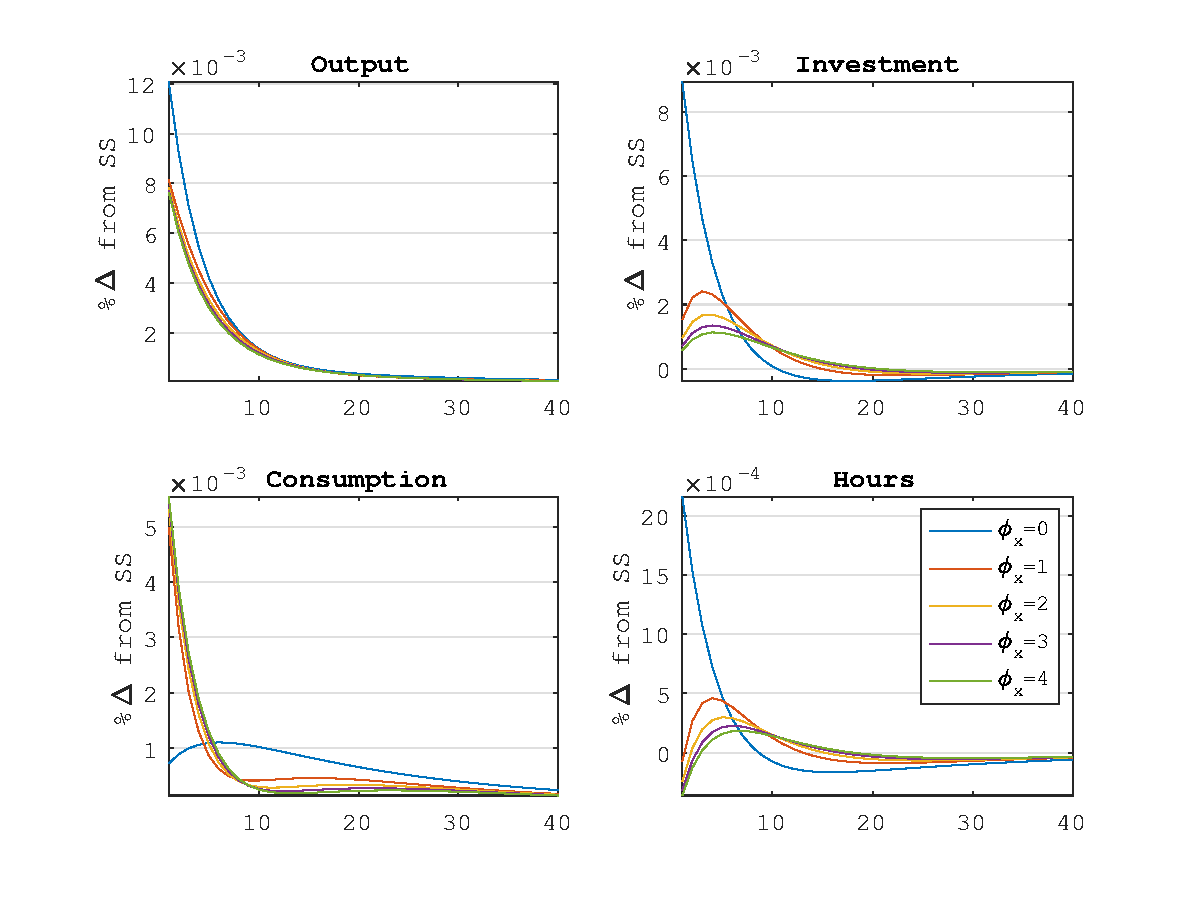
\includegraphics[width=0.8\linewidth]{IRFs}
  \caption{IRFs to different values for $\phi_x$}
  \label{thetay}
\end{figure}



\end{document}